\section{Architecture}

After a research and the first POC, I designed an architecture for the system. I considered all the use cases, the technical nature of the platform and technologies.

The \ref{fig:comp_arch} figure shows this architecture.

\begin{figure}[h]
    \centering
    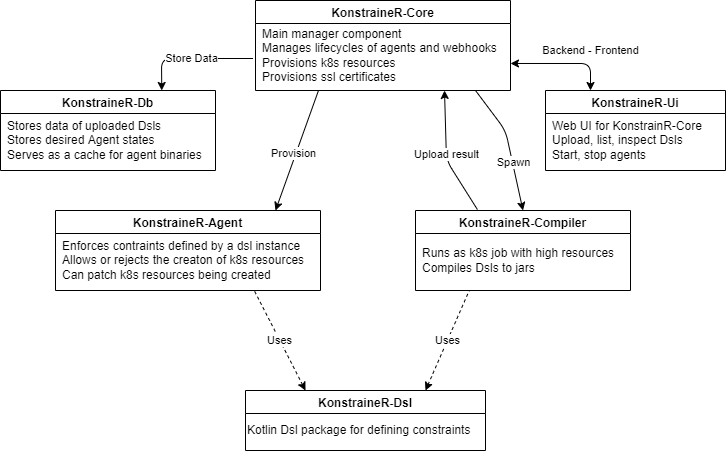
\includegraphics[width=130mm, keepaspectratio]{content/75_archPlan/xarch.png}
    \caption{Complex architecture plan}
    \label{fig:comp_arch}
\end{figure}


The main component in this setup is the KonstraineR-Core. This is an HTTP API server managing the whole application. DSL instances can be uploaded to it, and serves as a store for the uploaded and compiled DSL instances. It handles all tasks related to spawning, starting, configuring, and destroying agents. Most importantly it manages the TLS certificates and webhooks, which are crucial parts of the agent lifecycle management.

In Kubernetes, webhooks need to communicate with the Kubernetes API on a secured connection. To achieve this, KonstraineR-Agent instances require a TLS certificate, and need to serve request using the HTTPS protocol. This certificate can be self signed, but in the webhook creation request the CA Key of the certificate must be sent to the Kubernetes API for signing. After this, the Kubernetes API will trust the certificate of the webhook.

The mutating or validation webhooks have their own Kubernetes resource. It is either a \emph{MutatingWebhookConfiguration} or a \emph{ValidatingWebhookConfiguration}. These need to be created in the cluster, so Kubernetes can send the object creation requests to the Pod implementing the webhook.

After the webhook is configured and created in Kubernetes, the Agent can be spawned. Agents are spawned as \emph{deployment}s and they also require a \emph{service}. There are two complicated tasks with the creation of the deployment. First the a TLS certificate must be mounted to the Agent container. Second, the compiled DSL must be also mounted to the container. At this point I haven't decided what is the best way to achieve this. Automated Agent spawning is not the scope of this semester. For now, I styed with copying the required files to the Agent container by hand.

When an Agent is deleted there is a cleanup job to do. All the created Kubernetes resources associated with the given Agent must be deleted alongside with the \emph{WebhookConfiguration}. The deletion of the \emph{deployment}, \emph{service} and \emph{WebhookConfiguration} must be atomic.

The status of the DSL instance represents the compilation state of the instance, whether it is being compiled, successfully compiled, or outdated and needs to be recompiled.

Caching the compiled DSL instances is very important. A DSL instances are compiled to JVM byte code using gradle, so compilation can take long. Compiling a DSL before each launch of an agent would significantly increase the startup time of the agent. A long startup time would mean a relatively long outage when the pod of an already existing agent gets destroyed. This could happen for many reasons, such as the pod gets evicted, deleted manually by an administrator or just simply encounters a fatal error.

An agent is a webserver that runs a DSL instance and implements a webhook. The core component spawns an agent for each deployed DSL instance.

The agent is implemented as a lightweight Ktor server. It loads a compiled Dsl class at startup time. The configuration of the agent is done by the core component.

The compilation task must be decoupled from the other components, because it is a short, but resource intensive task. Keeping it together with either the core or the agent would not be wise, since they are relatively lightweight components, requiring at most 128 MiB RAM and 100m CPU time each. Increasing the resources allocated for these components would waste expensive resources on the node. Keeping them low would result in very slow compilation times, or OOMKilled errors for the components compiling the DSL. An OOMKilled status means that the Pod tried to use more memory than its limit.


The KonstraineR-Dsl is an easy to use, highly extendible and expressive domain specific language designed to define rules and constraints in Kubernetes cluster, implemented as a software module.